\documentclass[border=10pt]{standalone}

\usepackage{tikz}
\usepackage{tikzsymbols}
\usetikzlibrary{calc,patterns,shapes.geometric}

\def\centerarc[#1](#2)(#3:#4:#5){\draw[#1] ($(#2)+({#5*cos(#3)},{#5*sin(#3)})$) arc (#3:#4:#5);}

\begin{document}
	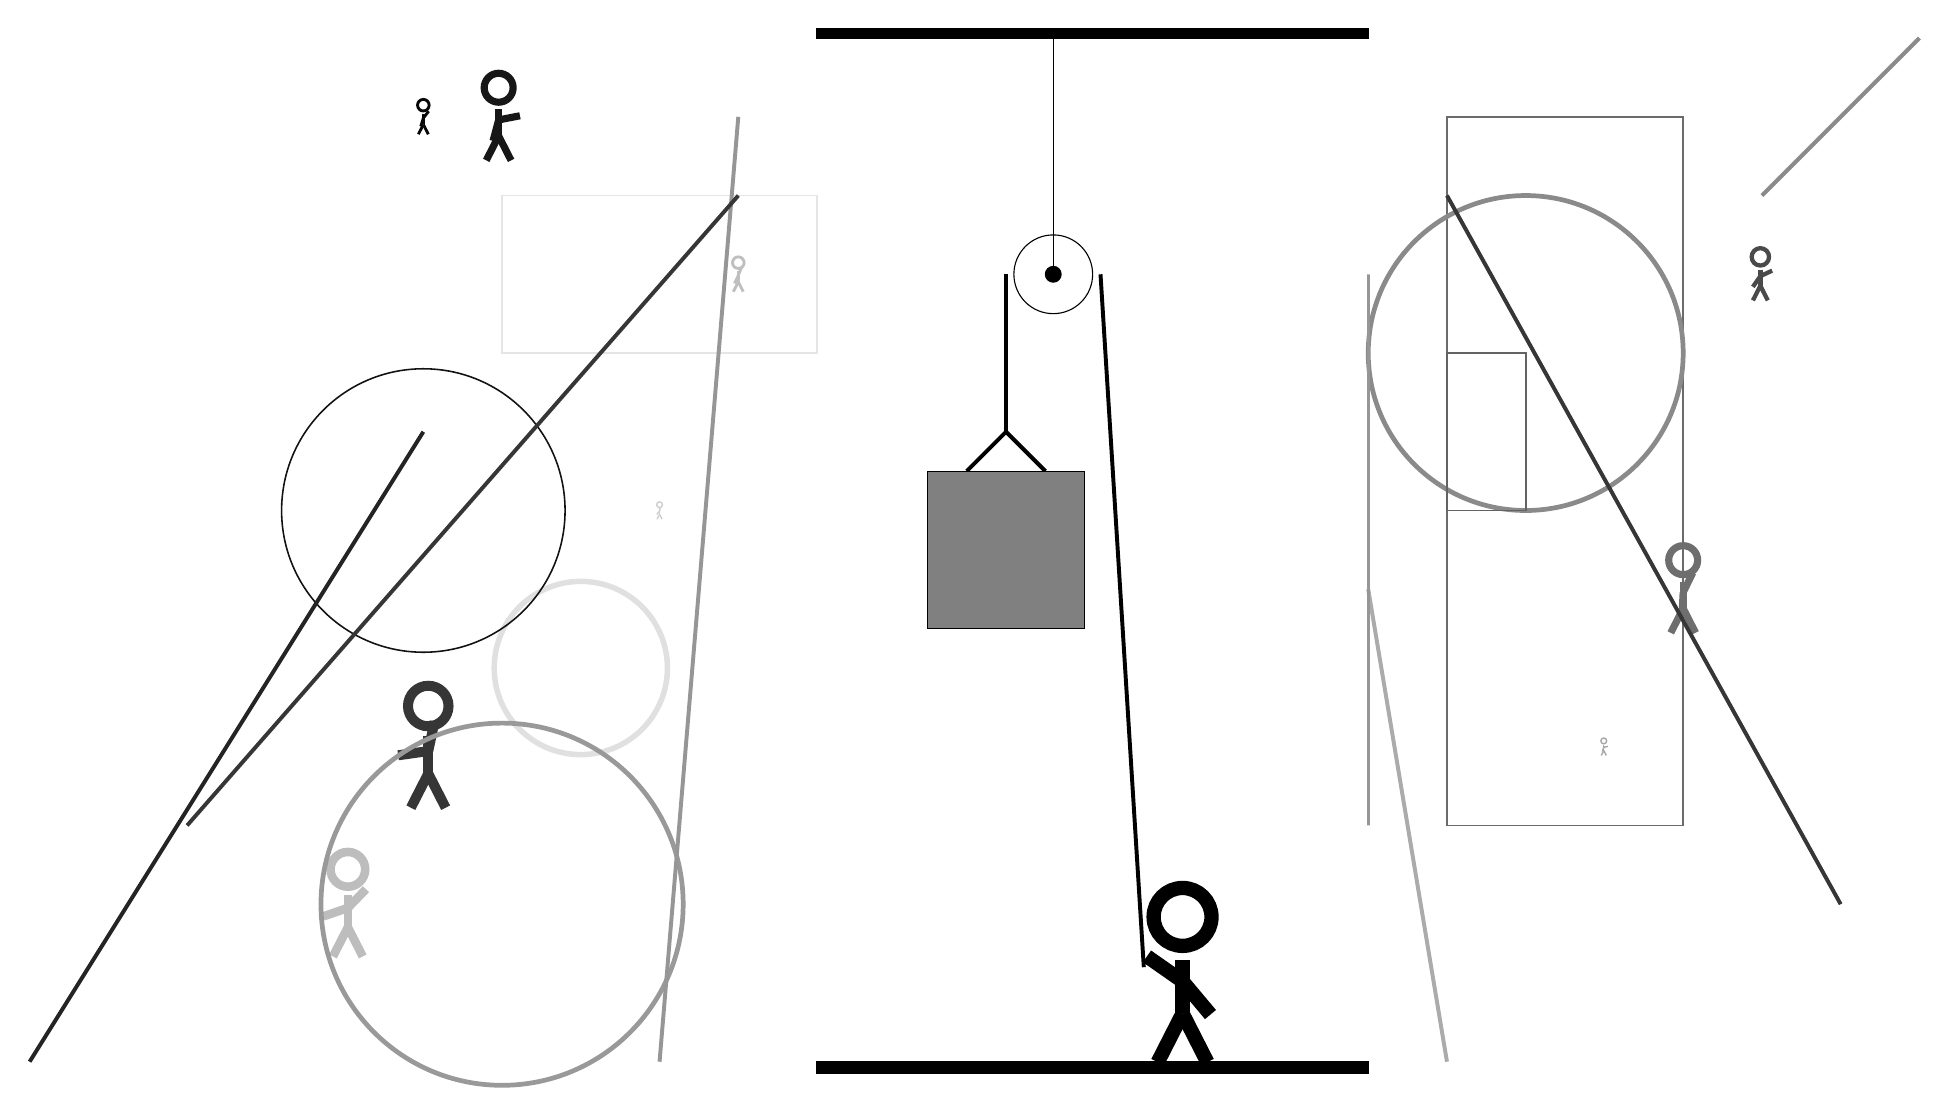
\begin{tikzpicture}
		%%%%% START %%%%%
		
		\draw[fill=black] (-2, 10) rectangle (5, 10.125);
		
		\draw (1, 7) circle (0.5);
		\draw[fill=black] (1, 7) circle (0.1);
		\draw (1, 10) -- (1, 7);
		
		\draw [line width=0.7mm, color=black!12](-5, 2) circle (1.1);
		
		\draw [line width=0.2mm, color=black!93](-7, 4) circle (1.8);
		\draw[line width=0.5mm, color=black!33](6, -3) -- (5, 3);
		\node[line width=0.4mm, color=black!26] at (-8, -1) {\Strichmaxerl[6][19][46]};
		\node[line width=0.5mm, color=black!79] at (-7, 1) {\Strichmaxerl[7][8][78]};
		
		\node[line width=0.3mm, color=black!34] at (8, 1) {\Strichmaxerl[1][71][14]};
		
		\draw[line width=0.2mm, color=black!58] (6, 9) rectangle (9, 0);
		\draw [line width=0.6mm, color=black!46](7, 6) circle (2.0);
		\draw[line width=0.2mm, color=black!10] (-2, 8) rectangle (-6, 6);
		
		\node[line width=0.4mm, color=black!57] at (9, 3) {\Strichmaxerl[5][87][64]};
		
		\node[line width=0.7mm, color=black!97] at (-7, 9) {\Strichmaxerl[2][73][52]};
		
		\node[line width=0.7mm, color=black!91] at (-6, 9) {\Strichmaxerl[5][75][11]};
		\node[line width=0.5mm, color=black!25] at (-3, 7) {\Strichmaxerl[2][64][69]};
		\draw[line width=0.2mm, color=black!61] (6, 4) rectangle (7, 6);
		\draw [line width=0.6mm, color=black!40](-6, -1) circle (2.3);
		\draw[line width=0.5mm, color=black!86](-7, 5) -- (-12, -3);
		\draw[line width=0.4mm, color=black!41] (5, 0) rectangle (5, 7);
		
		\draw[line width=0.5mm, color=black!41](-3, 9) -- (-4, -3);
		\draw[line width=0.5mm, color=black!79](6, 8) -- (11, -1);
		\node[line width=0.4mm, color=black!71] at (10, 7) {\Strichmaxerl[3][55][25]};
		\node[line width=0.4mm, color=black!19] at (-4, 4) {\Strichmaxerl[1][49][78]};
		
		\draw[line width=0.5mm, color=black!46](10, 8) -- (12, 10);
		
		\draw[line width=0.5mm, color=black!79](-3, 8) -- (-10, 0);
		
		\draw[line width=0.5mm] (-0.1, 4.5) -- (0.4, 5.0) -- (0.9, 4.5);
		\draw[fill=black!50] (-0.6, 4.5) rectangle (1.4, 2.5);
		
		\draw[line width=0.5mm] (0.4, 7) -- (0.4, 5.0);
		\centerarc[line width=0.5mm](1, 7)(0:180:0.6);
		\draw[line width=0.5mm](1.6, 7) -- (2.15, -1.8);
		
		\node at (2.6, -1.9) {\Strichmaxerl[10][-35][-50]};
		
		\draw[fill=black] (-2, -3) rectangle (5, -3.15);
		
		%%%%% END %%%%%
	\end{tikzpicture}
\end{document}